\documentclass[]{book}
\usepackage{lmodern}
\usepackage{amssymb,amsmath}
\usepackage{ifxetex,ifluatex}
\usepackage{fixltx2e} % provides \textsubscript
\ifnum 0\ifxetex 1\fi\ifluatex 1\fi=0 % if pdftex
  \usepackage[T1]{fontenc}
  \usepackage[utf8]{inputenc}
\else % if luatex or xelatex
  \ifxetex
    \usepackage{mathspec}
  \else
    \usepackage{fontspec}
  \fi
  \defaultfontfeatures{Ligatures=TeX,Scale=MatchLowercase}
\fi
% use upquote if available, for straight quotes in verbatim environments
\IfFileExists{upquote.sty}{\usepackage{upquote}}{}
% use microtype if available
\IfFileExists{microtype.sty}{%
\usepackage{microtype}
\UseMicrotypeSet[protrusion]{basicmath} % disable protrusion for tt fonts
}{}
\usepackage[margin=1in]{geometry}
\usepackage{hyperref}
\hypersetup{unicode=true,
            pdftitle={Predictive Modeling with Trees},
            pdfauthor={Homer White},
            pdfborder={0 0 0},
            breaklinks=true}
\urlstyle{same}  % don't use monospace font for urls
\usepackage{natbib}
\bibliographystyle{apalike}
\usepackage{graphicx,grffile}
\makeatletter
\def\maxwidth{\ifdim\Gin@nat@width>\linewidth\linewidth\else\Gin@nat@width\fi}
\def\maxheight{\ifdim\Gin@nat@height>\textheight\textheight\else\Gin@nat@height\fi}
\makeatother
% Scale images if necessary, so that they will not overflow the page
% margins by default, and it is still possible to overwrite the defaults
% using explicit options in \includegraphics[width, height, ...]{}
\setkeys{Gin}{width=\maxwidth,height=\maxheight,keepaspectratio}
\IfFileExists{parskip.sty}{%
\usepackage{parskip}
}{% else
\setlength{\parindent}{0pt}
\setlength{\parskip}{6pt plus 2pt minus 1pt}
}
\setlength{\emergencystretch}{3em}  % prevent overfull lines
\providecommand{\tightlist}{%
  \setlength{\itemsep}{0pt}\setlength{\parskip}{0pt}}
\setcounter{secnumdepth}{5}
% Redefines (sub)paragraphs to behave more like sections
\ifx\paragraph\undefined\else
\let\oldparagraph\paragraph
\renewcommand{\paragraph}[1]{\oldparagraph{#1}\mbox{}}
\fi
\ifx\subparagraph\undefined\else
\let\oldsubparagraph\subparagraph
\renewcommand{\subparagraph}[1]{\oldsubparagraph{#1}\mbox{}}
\fi
\usepackage{booktabs}

%%% Use protect on footnotes to avoid problems with footnotes in titles
\let\rmarkdownfootnote\footnote%
\def\footnote{\protect\rmarkdownfootnote}

%%% Change title format to be more compact
\usepackage{titling}

% Create subtitle command for use in maketitle
\newcommand{\subtitle}[1]{
  \posttitle{
    \begin{center}\large#1\end{center}
    }
}

\setlength{\droptitle}{-2em}
  \title{Predictive Modeling with Trees}
  \pretitle{\vspace{\droptitle}\centering\huge}
  \posttitle{\par}
  \author{Homer White}
  \preauthor{\centering\large\emph}
  \postauthor{\par}
  \predate{\centering\large\emph}
  \postdate{\par}
  \date{2016-06-21}

\begin{document}
\maketitle

{
\setcounter{tocdepth}{1}
\tableofcontents
}
\chapter{Introduction}\label{introduction}

Let's see what we can do. Let's cite \citep{statlearn}.

\section{Graphs}\label{graphs}

Can we really make a graph with captions, and refer to it?

\begin{figure}

{\centering 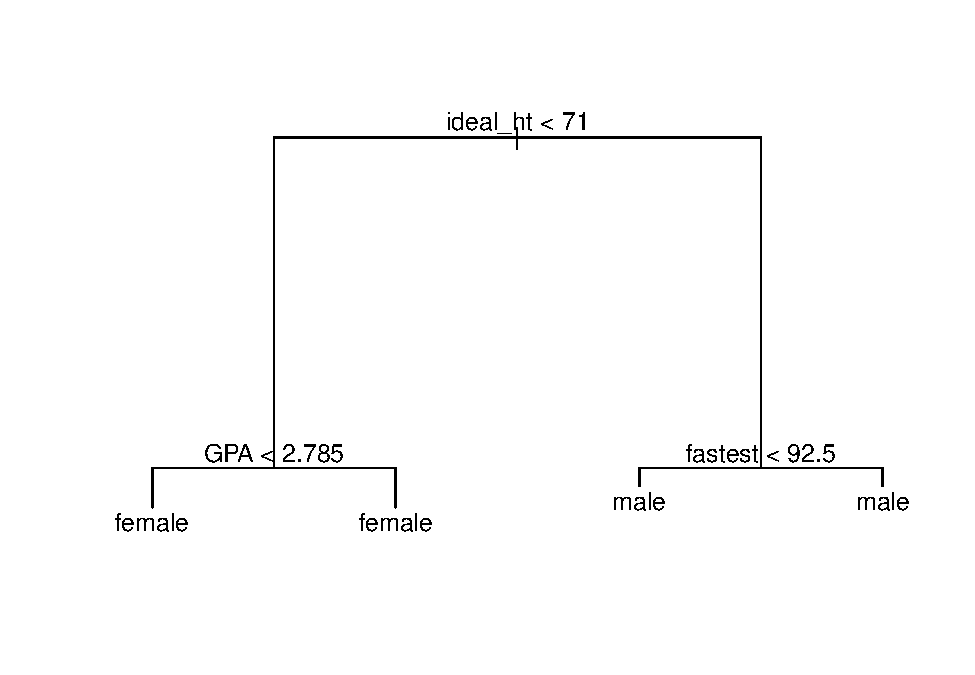
\includegraphics{bookdown-demo_files/figure-latex/ch1sextree-1} 

}

\caption{Default classification tree to predict sex on the basis of other variables in the `m111survey` data frame.}\label{fig:ch1sextree}
\end{figure}

As Figure \ref{fig:ch1sextree} shows \ldots{}

\section{Tables}\label{tables}

Hmm, let's make a table.\footnote{Tables are fun.}

\begin{table}

\caption{\label{tab:ch1sexconfusion}Confusion matrix for the tree model.}
\centering
\begin{tabular}[t]{l|r|r}
\hline
  & female & male\\
\hline
female & 37 & 2\\
\hline
male & 1 & 28\\
\hline
\end{tabular}
\end{table}

As Table \ref{tab:ch1sexconfusion} shows \ldots{}

We can learn about trees in Chapter \ref{randomforests}.

\chapter{Classification Trees}\label{classification-trees}

\chapter{Regression Trees}\label{regression-trees}

\chapter{Growing and Testing Trees for Predictive
Modeling}\label{growing-and-testing-trees-for-predictive-modeling}

\chapter{Random Forests: an Introduction}\label{randomforests}

\begin{rmdwarning}
Consider yourself warned.
\end{rmdwarning}

\bibliography{packages.bib,book.bib}


\end{document}
